%%%%%%%%%%%%%%%%%%%%%%%%%%%%%%%%%%%%%%%%%
% Long Professional Curriculum Vitae
% LaTeX Template
% Version 1.1 (9/12/12)
%
% This template has been downloaded from:
% http://www.latextemplates.com
%
% Original author:
% Rensselaer Polytechnic Institute (http://www.rpi.edu/dept/arc/training/latex/resumes/)
%
% Important note:
% This template requires the res.cls file to be in the same directory as the
% .tex file. The res.cls file provides the resume style used for structuring the
% document.
%
%%%%%%%%%%%%%%%%%%%%%%%%%%%%%%%%%%%%%%%%%

%----------------------------------------------------------------------------------------
% PACKAGES AND OTHER DOCUMENT CONFIGURATIONS
%----------------------------------------------------------------------------------------

\let\nofiles\relax
\documentclass{res}[12pt] % Use the res.cls style

% the font size can be changed to 11pt or 12pt
% -------------------------------------------------------------------------
% Font

%\usepackage{helvet}
%\renewcommand{\familydefault}{\sfdefault}
%\usepackage{CormorantGaramond}
\usepackage{fontspec}
\setmainfont{Avenir Next}[BoldFont={Avenir Next Demi Bold}]

\usepackage{fontmfizz}
\usepackage{fontawesome5}
\usepackage{cvicons}

\usepackage{graphicx}
\usepackage[official]{eurosym}
\usepackage{wrapfig}
\usepackage[hidelinks]{hyperref}
\usepackage{caption}
\captionsetup[figure]{labelformat=empty}

% -------------------------------------------------------------------------
% Bib

%\usepackage[style=numeric,sorting=ydnt,defernumbers,maxbibnames=20]{biblatex}
% \addbibresource{publications.bib}
%\AtEveryBibitem{\clearfield{url}}

% -------------------------------------------------------------------------
% Colors

\usepackage{xcolor}
% Define colors for social media links
\definecolor{email}{RGB}{0, 0, 0}
\definecolor{github}{RGB}{36, 41, 46}
\definecolor{youtube}{RGB}{255, 0, 0}
\definecolor{linkedin}{RGB}{0, 119, 181}
\definecolor{attachment}{HTML}{121b33}

\definecolor{flatBlue}{HTML}{3498db}
\definecolor{flatGreen}{HTML}{2ecc71}
\definecolor{flatRed}{HTML}{e74c3c}

\definecolor{skillbg}{HTML}{CCCCCC}
\definecolor{skillbar1}{HTML}{333333}
\definecolor{skillbar2}{HTML}{555555}
\definecolor{skillbar3}{HTML}{777777}
\definecolor{skillbar4}{HTML}{999999}
\definecolor{skillbar5}{HTML}{BBBBBB}

\definecolor{myBlue}{HTML}{121b33}
\definecolor{myWhite}{HTML}{f3f5ef}

\definecolor{skillFull}{HTML}{121b33}
\definecolor{skillEmpty}{HTML}{121b33}

% Change Bold Font Color
% \let\originaltextbf\textbf
% \renewcommand{\textbf}[1]{{\color{myBlue}\originaltextbf{#1}}}

% -------------------------------------------------------------------------
% Custom Commands

% Format entries takes 3 arguments: Title, Description, Date
\newcommand{\rEntry}[3]{%
  {\large\textbf{#1}} \hfill {\large\textbf{#3}} \\ % Degree and Year
  {\large#2} \vspace{0.3em} % Description
}
% Alternative entry format: takes w arguments: Title, Date
\newcommand{\rEntryAlt}[2]{%
  {\large\textbf{#1}} \hfill {\large\textbf{#2}} % Degree and Year
  \vspace{0.3em}
}
% Change section style
\newcommand{\rSection}[1]{\section{\Large\centerline{#1}}}
% Horizontal lines to separate sections
\newcommand{\sectionRule}{%
  {\vspace{20pt} \color{black} \hrule height 1.0pt}
}
% Attachment icon
\newcommand{\attachment}{\textcolor{attachment}{\hspace{1pt}\faFile}}
\newcommand{\mathematica}{\raisebox{-0.1em}{\textcolor{myBlue}{
\includegraphics[width=1em]{figures/mathematica_black.pdf}}}}

% -------------------------------------------------------------------------
% Hyperlinks

\hypersetup{
    colorlinks=true,
    linkcolor=flatBlue,
    filecolor=flatGreen,      
    urlcolor=flatRed,
    citecolor=flatBlue,
}

% -------------------------------------------------------------------------
% Packages

\usepackage{longtable}
\usepackage{tikz}
\usepackage{emoji}
\usepackage{tabularx}
\usepackage{comment}
\usepackage{enumitem}
%\usepackage{multicol}

% -------------------------------------------------------------------------
% Tikz

\usetikzlibrary{shapes.misc}

\newcommand{\skillbar}[1]{%
  \begin{tikzpicture}[scale=0.55, transform shape, minimum width=5mm, minimum height=2mm]
    \foreach \x in {1,2,3,4,5}{
      \ifnum\x>#1
        \draw [draw=skillEmpty, fill=none, line width=1.5pt, rounded corners=3pt] (\x*1.15-1.15,0) rectangle (\x*1.15-0.05,0.4);
      \else
        \draw [draw=skillFull, fill=skillFull, line width=1.5pt, rounded corners=3pt] (\x*1.15-1.15,0) rectangle (\x*1.15-0.05,0.4);
      \fi
    }
  \end{tikzpicture}
}



\newsectionwidth{0pt} % Stops section indenting\
\pagestyle{plain}

\begin{document}
\color{myBlue}
\pagecolor{myWhite}

%----------------------------------------------------------------------------------------
% YOUR NAME AND ADDRESS(ES) SECTION
%----------------------------------------------------------------------------------------

\begin{figure}[htbp]
\begin{center}
%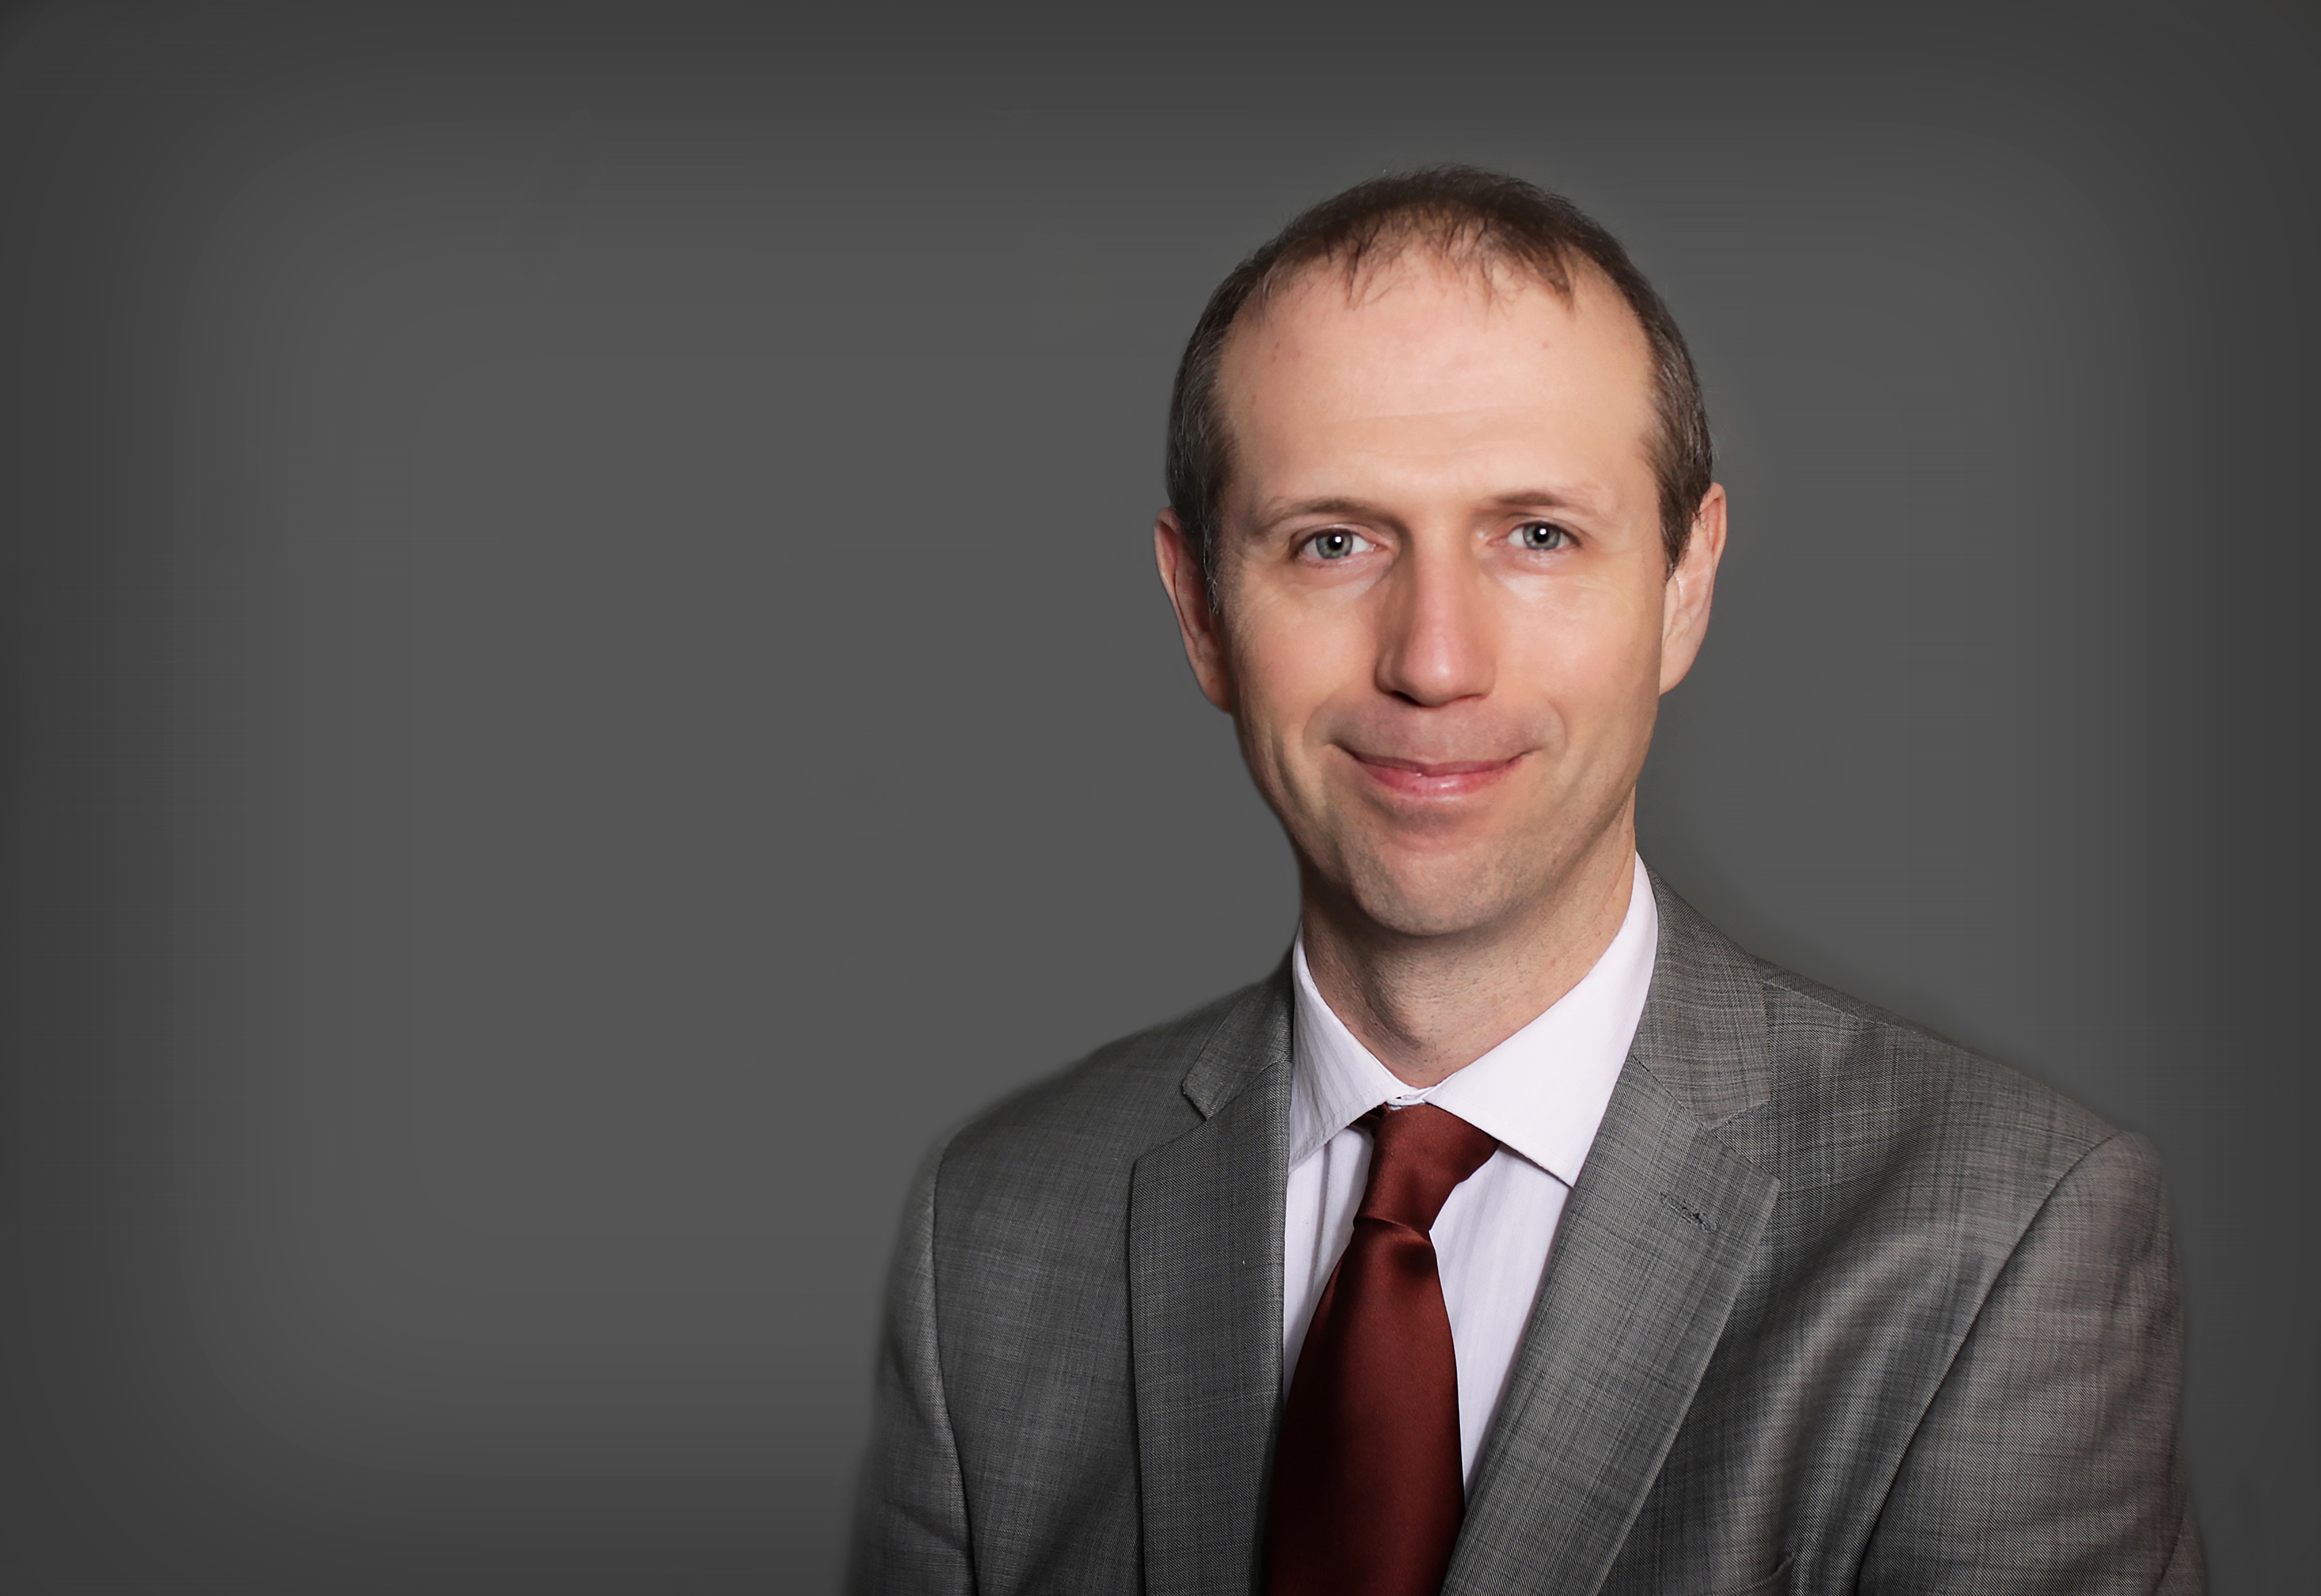
\includegraphics[width=0.125\textwidth]{figures/John.jpg}
\end{center}
\end{figure}

\name{\LARGE Jacopo Uggeri}% Your name at the top

% If you don't want one of the addresses, simply remove all the text in the first or second \address{} bracket

\address{{\large \bf Address} \\ 134-136 Cromwell Road \\ SW74HA \\ London \\ United Kingdom} % Your address 1

\address{{\large \bf Contact} \\
\href{mailto:jacopo.uggeri@gmail.com}{\textcolor{email}{jacopo.uggeri@gmail.com}} \\
\href{https://github.com/jacopouggeri}{\textcolor{github}{\faGithub\ GitHub}} \\
\href{https://www.youtube.com/@jacopouggeri}{\textcolor{youtube}{\faYoutube\ YouTube}} \\
\href{https://www.linkedin.com/in/jacopo-uggeri-191605198}{\textcolor{linkedin}{\faLinkedin\ LinkedIn}}} % Contact Information


%----------------------------------------------------------------------------------------

\begin{resume}

%----------------------------------------------------------------------------------------
% SUMMARY SECTION
%----------------------------------------------------------------------------------------

\rSection{\faClipboard \hspace{3pt} Summary}
\sectionRule
\vspace{6pt} % Gap between title and text

\large{I am a curiosity driven and passionate student with a strong interest in theoretical physics and cosmology. I am currently studying for a Master's degree in Physics with Theoretical Physics at Imperial College London. I am looking for a PhD position in Theoretical Physics, starting in 2023. Outside of physics, my interests extend to computer science, machine learning, and graphic design.}

%----------------------------------------------------------------------------------------
% PROFESSIONAL EXPERIENCE SECTION
%----------------------------------------------------------------------------------------

\rSection{\faBriefcase \hspace{3pt} Professional Experience}
\sectionRule
\vspace{6pt} % Gap between title and text

% \begin{itemize} \itemsep -2pt % Reduce space between items
% \end{itemize}

\rEntry{Graduate Teaching Assistant}{
Department of Physics, Imperial College London (London), United Kingdom} {2022 -- 2023}

%----------------------------------------------------------------------------------------

% \vspace{0.2in} % Some whitespace between sections

%----------------------------------------------------------------------------------------
% EDUCATION SECTION
%----------------------------------------------------------------------------------------

\rSection{\faGraduationCap \hspace{3pt} Education}
\sectionRule
\vspace{6pt} % Gap between title and text

\rEntry{MSci Physics with Theoretical Physics}{Imperial College London (London), United Kingdom}{2019 -- present}

\begin{itemize} \itemsep -2pt
\item Attended a variety of courses that granted a solid foundation in scientific and critical thinking, with a focus on theoretical physics
\item Achieved 1st class in theoretical modules: Mathematical Methods, Foundations of Quantum Mechanics, Advanced Classical Physics, Group Theory, Nuclear and Particle Physics, Statistical Mechanics
\item Current relevant courses: Quantum Field Theory, Unification, General Relativity, Cosmology
\item Used Python extensively for data analysis of experiments and simulations
\end{itemize}

\rEntry{Diploma di Liceo Scientifico Tradizionale}{
Liceo Scientifico Giovanni Gandini (Lodi), Italy}{2013 -- 2019}
\begin{itemize} \itemsep -2pt
\item Scientifically oriented high school program with a wide range of subjects spanning both sciences and humanities
\item Participated in extracurricular events and activities with a focus on Physics and Mathematics
\item Graduated with 100/100 at \sl{Esame di Stato}
\end{itemize}


%----------------------------------------------------------------------------------------
 
% \vspace{0.2in} % Some whitespace between sections

%----------------------------------------------------------------------------------------
% PROJECTS SECTION
%----------------------------------------------------------------------------------------

\rSection{\faLaptopCode \hspace{3pt} Projects}
\sectionRule
\vspace{6pt} % Gap between title and text

\rEntry{Shining Light on Missing Red Giants: \\Red Giant Photoevaporation in the Galactic Centre \href{https://github.com/jacopouggeri/red_giant_photoevaporation.git}{\textcolor{github}{\faGithub}}}{MSci Project at Imperial College London}{2022 -- present}
\begin{itemize}
\item I determined the photo evaporation rate of red giants around supermassive black holes and determined how it affects their evolution, with the aim of explaining the observed lack of these stars compared to equilibrium theoretical predictions.
\item Computational and theoretical project: involved designing, writing and testing code that could be shared with others.
\item Helped develop critical scientific thinking and research skills.
\item The project reached positive and encouraging conclusions.
\end{itemize}

\rEntry{Search for beyond SM physics from LHCb data}{Group Project at Imperial College London}{2021}
\begin{itemize}
\item Involved coordinating with other \textasciitilde 20 students to analyze data from LHCb experiment.
\item Participated in group discussions and contributed meaningful ideas.
\item Main role was to train a decision tree model to separate background from signal.
\end{itemize}


\rEntry{Improving people counter image recognition neural network \href{https://github.com/jacopouggeri/curriculumVitae/blob/84ad9712112b11ea237b126a98ba1764b27054b4/attachments/grottini.pdf}{\attachment}}{Summer work experience at GrottiniLab with Politecnico di Ancona}{2020}
\begin{itemize}
\item Was assigned to a software engineer working on a "people counter" neural network, with the aim of exploring new avenues of improvement.
\item Reviewed literature on the current state of the art of image recognition neural networks.
\item Proposed and coded a new data augmentation strategy to improve the product.
\end{itemize}

\rEntry{Critical Temperature of an Ising Model on a Sierpinski Gasket}{Year 1 Summer Project at Imperial College London}{2020}
\begin{itemize}
\item Worked remotely with a peer to simulate an Ising model on a Sierpinski gasket network.
\item Wrote Python code to run, visualize and analyze the simulation, and numerically evaluated the model's critical temperature and the corresponding critical exponent.
\item Delivered a video summary of the project and a project report.
\end{itemize}


%----------------------------------------------------------------------------------------
 
% \vspace{0.2in} % Some whitespace between sections

%----------------------------------------------------------------------------------------
% EXPERIENCES SECTION
%----------------------------------------------------------------------------------------
\newpage
\rSection{\faStar \hspace{3pt} Experiences}
\sectionRule
\vspace{6pt} % Gap between title and text

\rEntry{DeepLearn Summer School \href{https://github.com/jacopouggeri/curriculumVitae/blob/84ad9712112b11ea237b126a98ba1764b27054b4/attachments/deeplearn.pdf}{\attachment}}{4th International School on Deep Learning}{2021}

\begin{itemize}
\item Attended 38 hours of postgraduate level lectures given by Machine Learning experts from various fields.
\item Learned to comprehend and acquire meaningful information from lectures that assumed more advanced background knowledge than I had.
\end{itemize}

\rEntry{Project Extreme Energy Events (EEE) \href{https://github.com/jacopouggeri/curriculumVitae/blob/84ad9712112b11ea237b126a98ba1764b27054b4/attachments/eee.pdf}{\attachment}}{Long running project organized by INFN involving multiple Italian high schools}{2013 -- 2019}
\begin{itemize}
\item Participated in the data taking and analysis process for a MRPC muon detector.
\item Attended lectures and conferences on particle Physics.
\item Participated in joint conferences between participating schools summarizing recent results.
\end{itemize}

\rEntryAlt{Building a MRPC muon detector chamber at CERN \href{https://github.com/jacopouggeri/curriculumVitae/blob/84ad9712112b11ea237b126a98ba1764b27054b4/attachments/eee.pdf}{\attachment}}{2017}
\begin{itemize}
\item Worked with peers in a laboratory to assemble a muon detector chamber.
\item Attended seminars hosted by CERN personnel regarding the present state of particle Physics.
\end{itemize}

%----------------------------------------------------------------------------------------
 
% \vspace{0.2in} % Some whitespace between sections

%----------------------------------------------------------------------------------------
% SKILLS SECTION
%----------------------------------------------------------------------------------------

\rSection{\faWrench \hspace{3pt} Skills}
\sectionRule
\vspace{6pt} % Gap between title and text

\subsection*{\faTerminal \hspace{3pt} Coding}

\begin{minipage}{0.49\textwidth}
    \begin{itemize}
        \large
        \item[\mfPython] Python \hfill\skillbar{5}
        \item[\mfJava] Java \hfill\skillbar{3}
        \item[\mfCplusplus] C++ \hfill\skillbar{2}
        \item[\mfHaskell] Haskell \hfill\skillbar{2}
        \item[\cvMathematica] Mathematica \hfill\skillbar{2}
        \item[\mfJavascriptAlt] JavaScript \hfill\skillbar{2}
    \end{itemize}
\end{minipage}
\hfill
\begin{minipage}{0.49\textwidth}
    \begin{itemize}
        \large
        \item[\mfRuby] Ruby \hfill\skillbar{2}
        \item[\mfHtmlfiveAlt] HTML \hfill\skillbar{4}
        \item[\TeX] LaTeX \hfill\skillbar{4}
        \item[\mfGit] Git \hfill\skillbar{3}
        \item[\mfShell] Shell \hfill\skillbar{3}
    \end{itemize}
\end{minipage}


\subsection*{\faGlobe \hspace{3pt} Languages}

\begin{minipage}{0.49\textwidth}
    \begin{itemize}
        \large
        \item[\emoji{flag-italy}] Italian \hfill\skillbar{5}
        \item[\emoji{flag-united-kingdom}] English \hfill\skillbar{5}
        \item[\emoji{flag-spain}] Spanish \hfill\skillbar{4}
    \end{itemize}
\end{minipage}
\hfill
\begin{minipage}{0.49\textwidth}
    \begin{itemize}
        \large
        \item[\emoji{flag-japan}] Japanese \hfill\hfill\skillbar{3}
        \item[\emoji{flag-china}] Mandarin \hfill\hfill\skillbar{1}
    \end{itemize}
\end{minipage}


\subsection*{Others}
\begin{itemize}
    \large
    \item[\faPalette] Adobe Suite: Illustrator, Photoshop, InDesign, Premiere Pro
    \item[\faCode] Machine Learning libraries: PyTorch, Keras, OpenCV
    \item[\faBrain] AI Prompt Engineering
    \item[\faBook] Independent Study
\end{itemize}

\rSection{\faAward \hspace{3pt} Achievements}
\sectionRule
\vspace{6pt} % Gap between title and text

{\large
\renewcommand{\arraystretch}{1.5}
\begin{tabularx}{\textwidth}{ p{200pt} X p{30pt} X }
     & \textbf{Where} & \textbf{Year} & \textbf{Award} \\
    Japanese Level 3 & Imperial Horizons & 2022 & Pass with Merit \\
    Jiu-Jitsu & Imperial Jiu-Jitsu & 2022 & Orange Belt \\
    Understanding the Nature of Science & Imperial Horizons & 2020 & Pass with Merit \\
    Aikido & Aikikai Carpiano & 2019 & 5th Kyu \\
\end{tabularx}
}

\begin{comment}
\newpage


\begin{minipage}{0.5\textwidth}
    \begin{tikzpicture}[x=1cm,y=0.8cm]
        \draw[thick,-stealth] (0,0) -- (0,20);
        \foreach \y/\year/\event/\description in {
            1/2016/Bachelor's Degree in Computer Science/{},
            3/2018/Internship at XYZ Company/{},
            5/2019/Master's Degree in Computer Science/{},
            7/2020/Research Assistant at University of ABC/{},
            9/2022/Software Developer at XYZ Company/{}
        } {
            \draw (0,\y) -- (-0.2,\y);
            \node[anchor=east, font=\small] at (-0.3,\y) {\year};
            \node[anchor=west, font=\small] at (0.3,\y) {\event};
            \node[anchor=west, text width=9cm, font=\footnotesize] at (1,\y) {\description};
        }
    \end{tikzpicture}
\end{minipage}
\hfill
\begin{minipage}{0.5\textwidth}
    % your text here
\end{minipage}

\end{comment}

%Personal Projects:
%Experimented with numerical simulations of PDEs
%Implemented and experimented with Cellular Automata: Game of Life, SmoothLife, Lenia, MNCA

%----------------------------------------------------------------------------------------

\vspace{0.2in} % Some whitespace between sections

\end{resume} 
\end{document}